% set 0 inch indentation
\setlength{\parindent}{0in}
% set paragraph space = 1 space
\setlength{\parskip}{1em}
% set line space 1.5
\setlength{\baselineskip}{1.6em}

\chapter{Methodology}
\label{ch:methodology}

The methodology of the proposed study can be separated into five main processes, as shown in Figure \ref{fig:system_overview} and as follows.
\begin{enumerate}
  \item Design and build a filter, amplifier, and embedded system to digitize and analyze signals from seismic sensors characterizing human activities.
  \item Collect data on daily human activities by many subjects.
  \item Build an anomaly detection and alerting system for detecting anomaly patterns. The target accuracy should be a 75\% hit rate for anomalous events.
  \item Deploy the model in the living room in my home.
  \item Evaluate the deployed model in terms of its accuracy in identifying unusual events.
  % \item Evaluate the deployed model in terms of its accuracy in identifying unusual events which should be less than 5 false positive per day.
\end{enumerate}

\begin{figure}[H]
  \centering
  \caption[Overview of the methodology.]{\emph{Overview of the methodology.}}\label{fig:system_overview}
  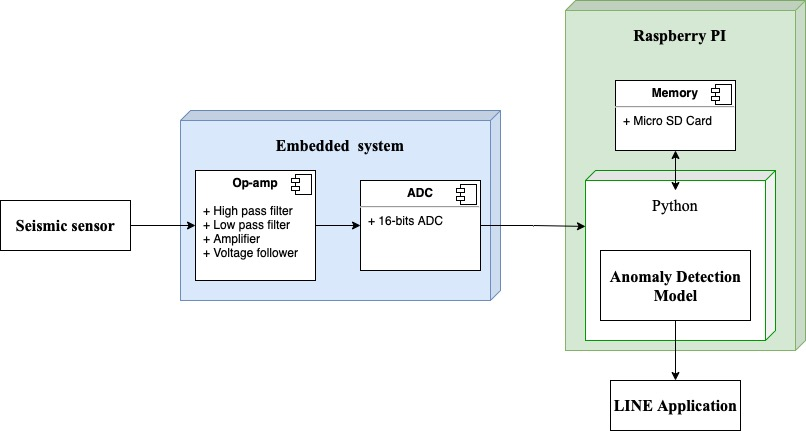
\includegraphics[scale = 0.5]{figures/system_overview_2.jpg}
\end{figure}

\begin{figure}[H]
  \centering
  \caption[Data collection - hardware.]{\emph{Data collection - hardware.}}\label{fig:data_collection}
  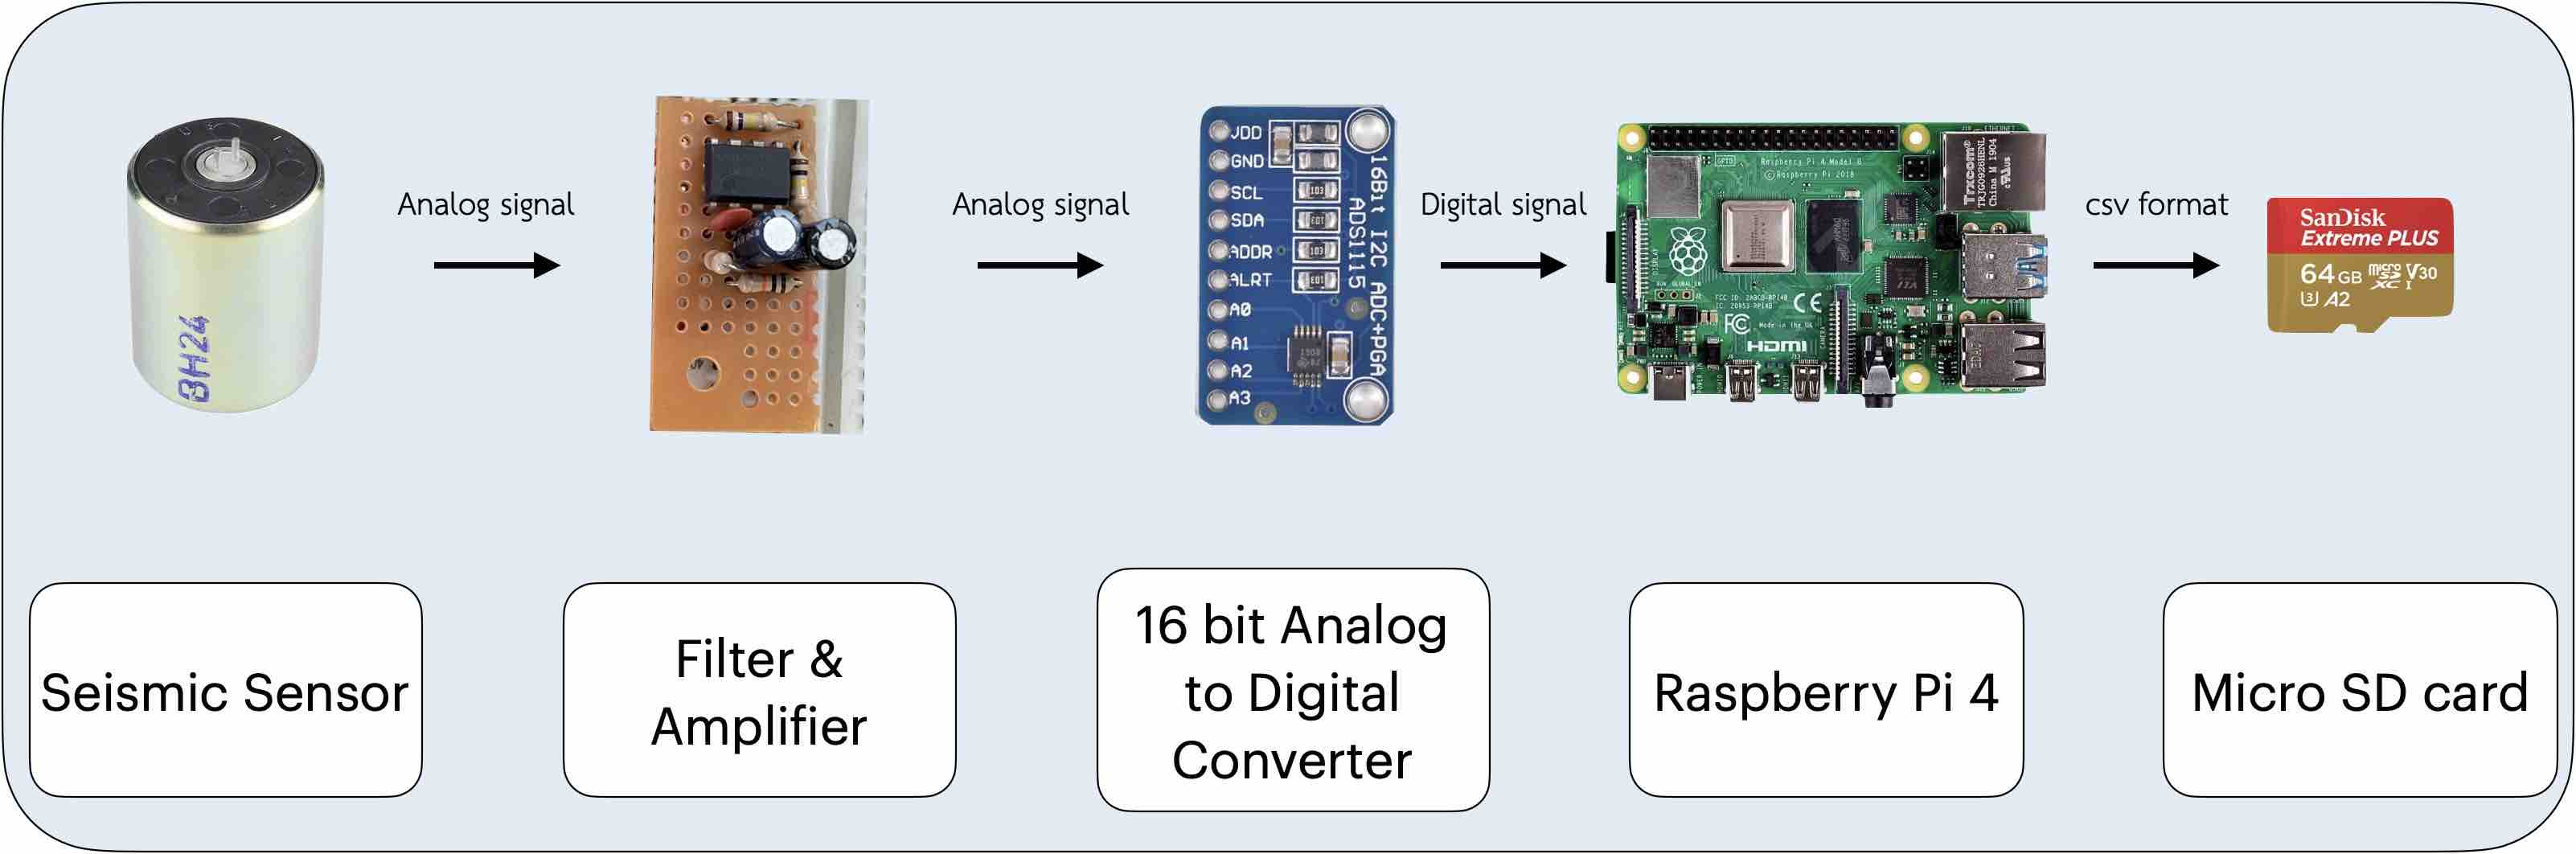
\includegraphics[scale = 0.13]{figures/meth_data_collection.jpg}
\end{figure}

\begin{figure}[H]
  \centering
  \caption[Training model process.]{\emph{Training model process.}}\label{fig:training}
  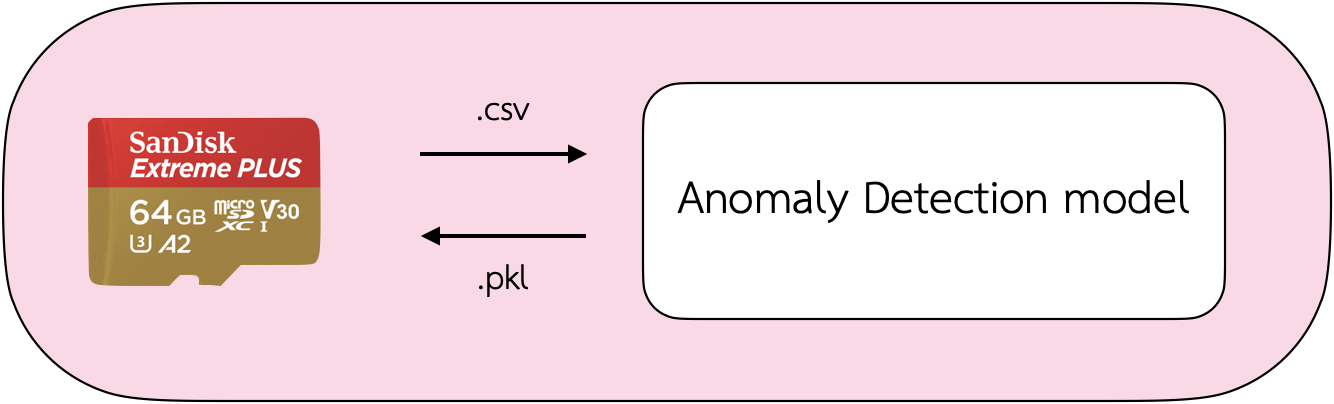
\includegraphics[scale = 0.2]{figures/meth_training.jpg}
\end{figure}

\begin{figure}[H]
  \centering
  \caption[Realtime deployment system - data flow diagram.]{\emph{Realtime deployment system - data flow diagram.}}\label{fig:deploy_data_flow}
  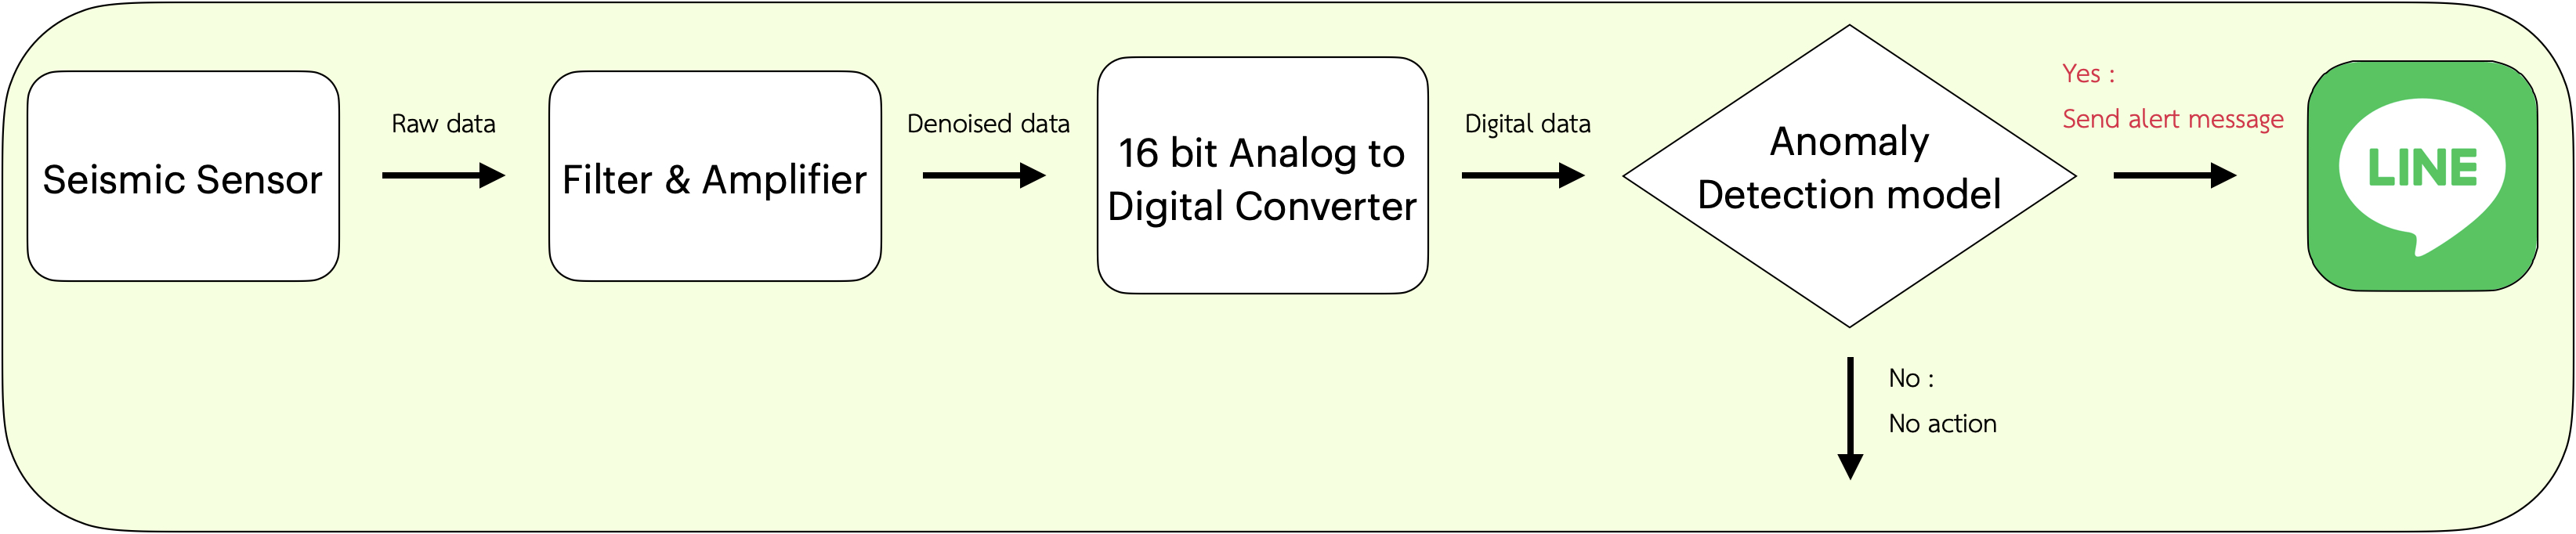
\includegraphics[scale = 0.13]{figures/meth_deploy.jpg}
\end{figure}


\section{Data Collection}

To collect raw data, we need to build a prototype embedded system. To detect human falls, we must simulate falls and other anomalous events along with ordinary activities. The embedded system must also be capable of collecting and recording the vibration signal over a long period of time.

\subsection{Hardware}

There are four significant hardware components, as shown in Figure \ref{fig:data_collection}. Each component has a specific propose.

\begin{figure}[h]
  \centering
  \caption[Hardware required to receive raw vibration signal data.]{\emph{Hardware required to receive raw vibration signal data. \\}}\label{fig:hardware}
  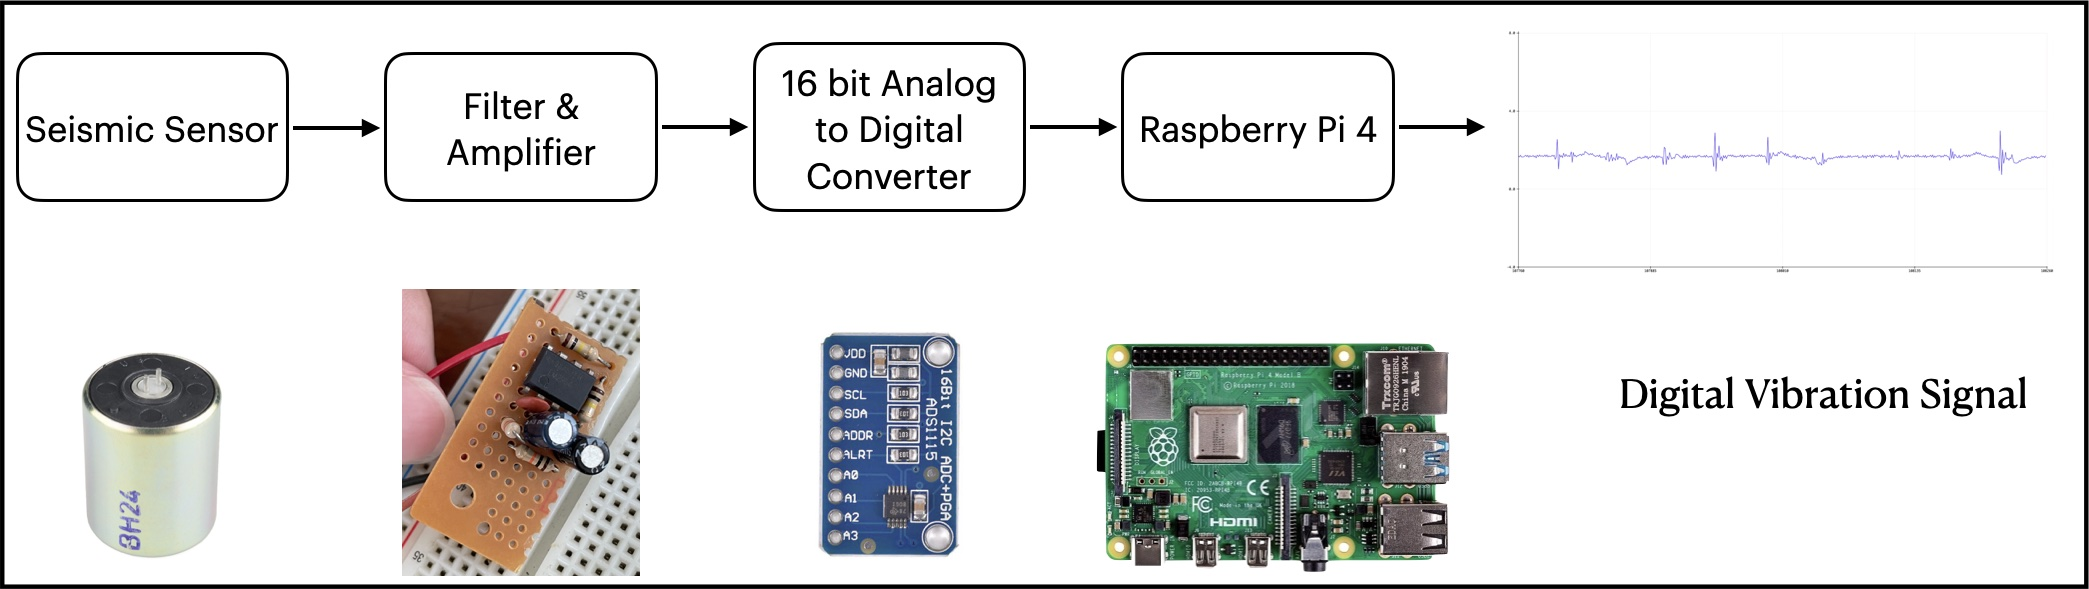
\includegraphics[scale = 0.2]{figures/hardware.jpg}
\end{figure}


The first main component is the seismic sensor or geophone shown in Figure \ref{fig:seismic}, A geophone is a device that converts ground vibration (velocity) into voltage. Geophones have historically been passive analog devices that typically comprise a spring-mounted wire coil moving within the field of a case-mounted permanent magnet to generate an electrical signal. I decided to use the geophone SM-24 because it has a small size, similar to a coin, and is easy to install by just setting it on the ground. However, the SM-24 cannot connect directly to a microcontroller because it generates voltage up to $28.8$ V (corresponding to $1$ m/s velocity of the coil). Therefore, we have designed an embedded system to convert the $0 - 28.8$ V range to the into range $0 - 5$ V.

\begin{figure}[H]
  \centering
  \caption[A geophone SM-24 and its interior elements.]{\emph{A geophone SM-24 and its interior elements. \\Reprinted from Sparkfun, (2017). }}\label{fig:seismic}
  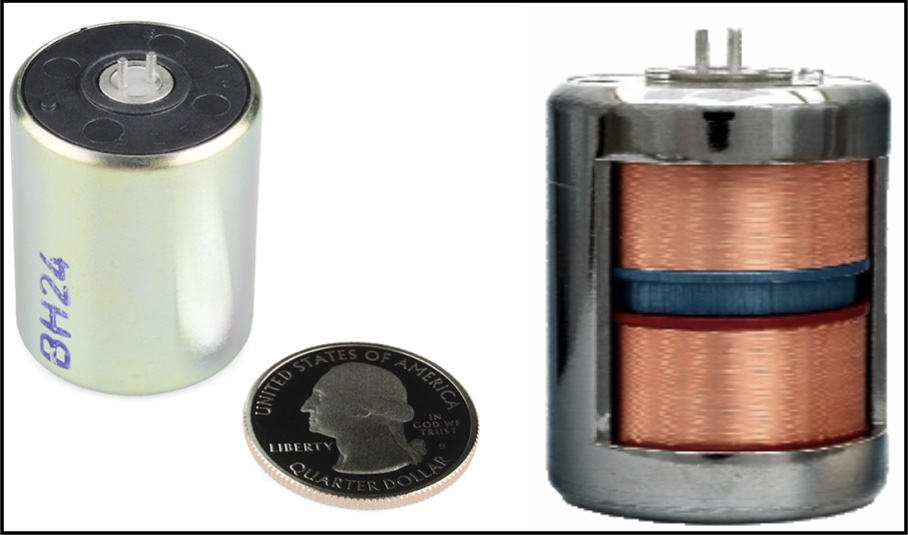
\includegraphics[scale = 0.3]{figures/seismic.jpg}
\end{figure}


The second main component is the analog circuit of the filter \& amplifier, which is shown in Figure \ref{fig:analog_circuit}, has four significant logical components, as a DC offset, a high-pass filter (HPF), an amplifier, and a low-pass filter (LPF). The DC offset is used for set the reference signal as 2.5 V. The HPF eliminates any frequencies below the frequency range of interest. It has an ideal cutoff frequency around 100 Hz. The amplifier provides a high voltage gain of around 200 to prepare for sampling at a high resolution at the analog to digital converter (ADC). Lastly, the low-pass filter has a cut-off frequency at 100 kHz, making the overall frequency range of interest 100 - 100 kHz. However, this is a first prototype, and the goal is 0 - 200 Hz.

\begin{figure}[H]
  \centering
  \caption[Analog circuit measure vibrations caused by human activity.]{\emph{Analog circuit measure vibrations caused by human activity.}}\label{fig:analog_circuit}
  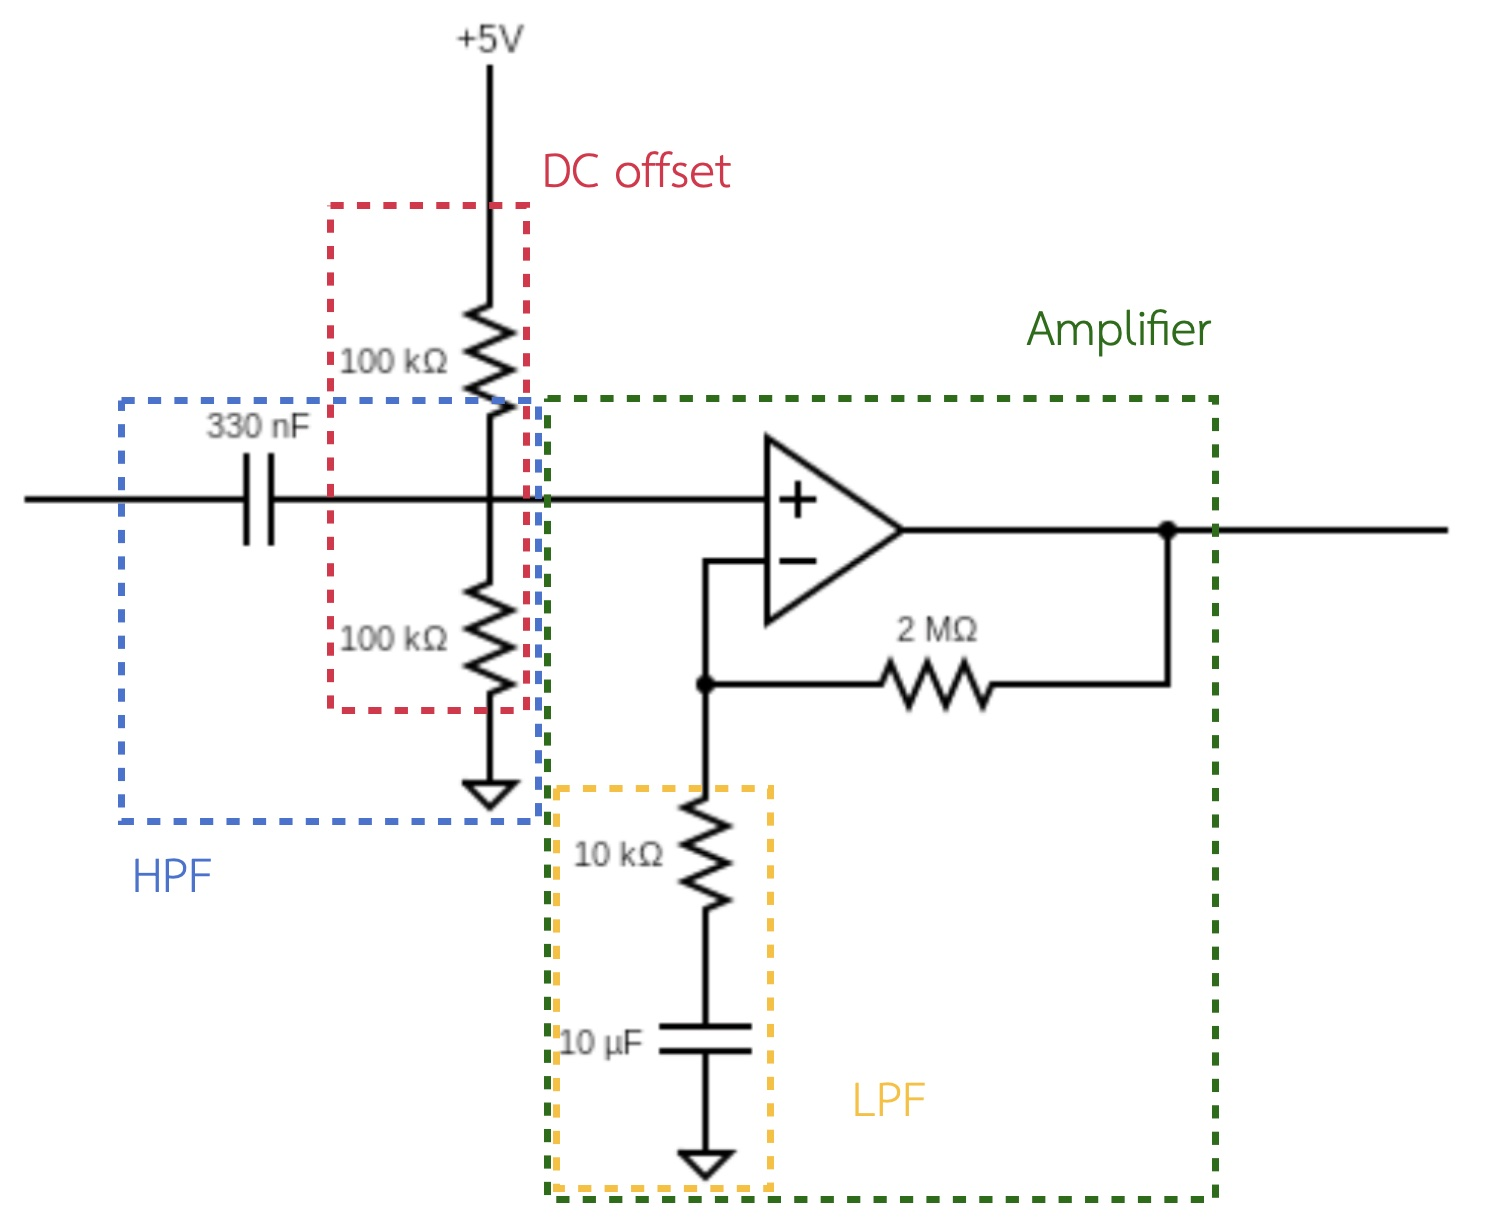
\includegraphics[scale = 0.2]{figures/analogcircuit.jpg}
\end{figure}


The third main component is analog to digital converter (ADC), Higher bit width means a filter that can represents the data stream more accurately. Figure \ref{fig:adc} provides the intuition behind the difference between a 10-bit and 16-bit ADC.  The red line shows a signal measured at 10 bits in the adc pin of the Arduino Mega, and the blue line shows the same original signal measured with a 16-bit ADC. After the raw analog signal is filtered and amplified, it needs to be sampled at a rate of 500 samples/second and quantized at a resolution of 16 bits/sample in order to prepare it for digital transmission. A 16-bit ADC is capable of distinguishing $65536$ ($2^{16}$) different voltage levels within a narrow voltage range from $0 - 5$ Volts. It means that each level represents approximately 76.3 uV, which is sufficient to capture accurate signals from the seismic sensor.

\begin{figure}[H]
  \centering
  \caption[Comparison 10-bit (red) and 16-bit (blue) ADC.]{\emph{Comparison 10-bit (red) and 16-bit (blue) ADC.}}\label{fig:adc}
  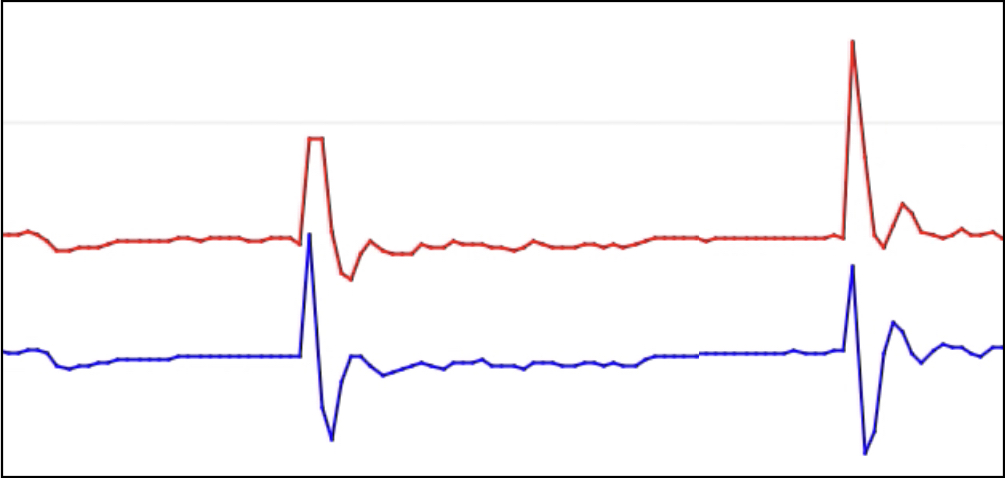
\includegraphics[scale = 0.3]{figures/ADC.jpg}
\end{figure}


The fourth main component, shown in Figure \ref{fig:pi4}, is the single-board, a Raspberry Pi 4 model B, which is a small size, low price system with several useful functions, and sufficient power for machine learning inference. The digital signal is fed from ADC to Raspbery Pi via I2C which is a synchronous serial communication interface specification used for short-distance communication. And then these raw signals are saved to the file system on a mircro SD card.

\begin{figure}[H]
  \centering
  \caption[Raspberry Pi 4 model B.]{\emph{Raspberry Pi 4 model B. \\ Reprinted from Raspbery Pi officially}}\label{fig:pi4}
  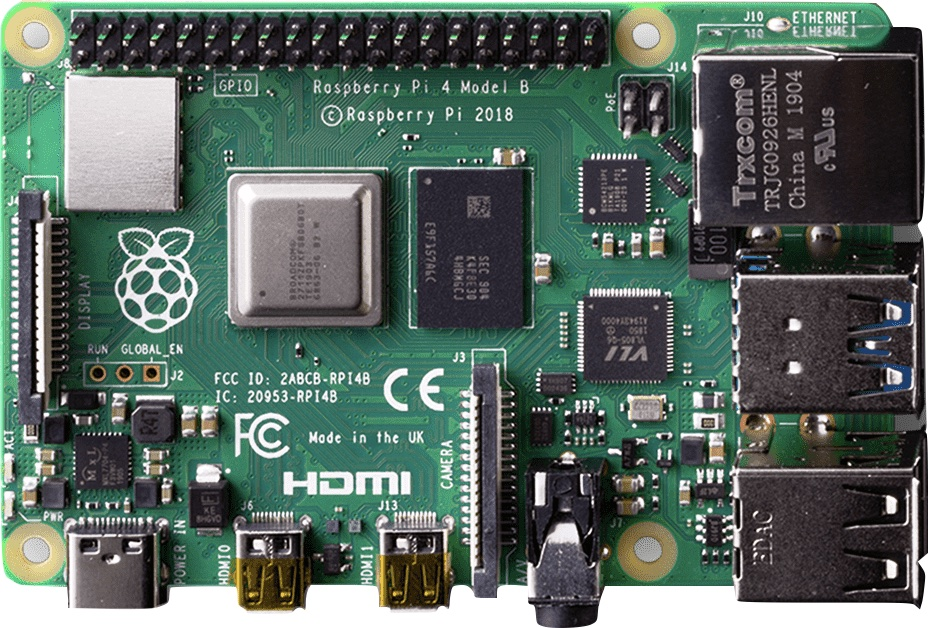
\includegraphics[scale = 0.14]{figures/pi4.jpg}
\end{figure}

\section{Anomaly Detection Models}

I choose two candidate models as autoencoder with LSTM architecture as shown in Figure \ref{fig:LSTM_metho} and the Transformer shown in Figure \ref{fig:transformer_metho}, which are both state of the art models for distinguishing abnormal event in sequencial data.

\begin{figure}[H]
  \centering
  \caption[The autoencoder with LSTM architecture (seq2seq structure).]{\emph{The autoencoder with LSTM architecture (SEQ2SEQ structure).}}\label{fig:LSTM_metho}
  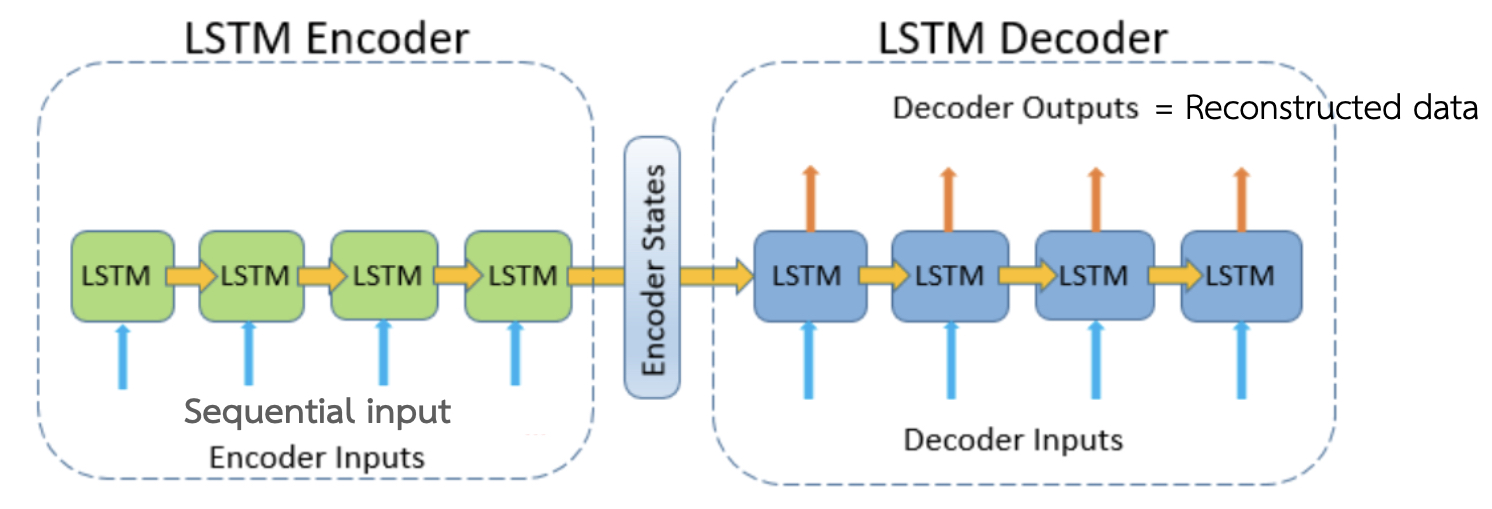
\includegraphics[scale = 0.3]{figures/LSTM_metho.jpg}
\end{figure}

\begin{figure}[H]
  \centering
  \caption[The Transformer architecture.]{\emph{The Transformer architecture. \\}}\label{fig:transformer_metho}
  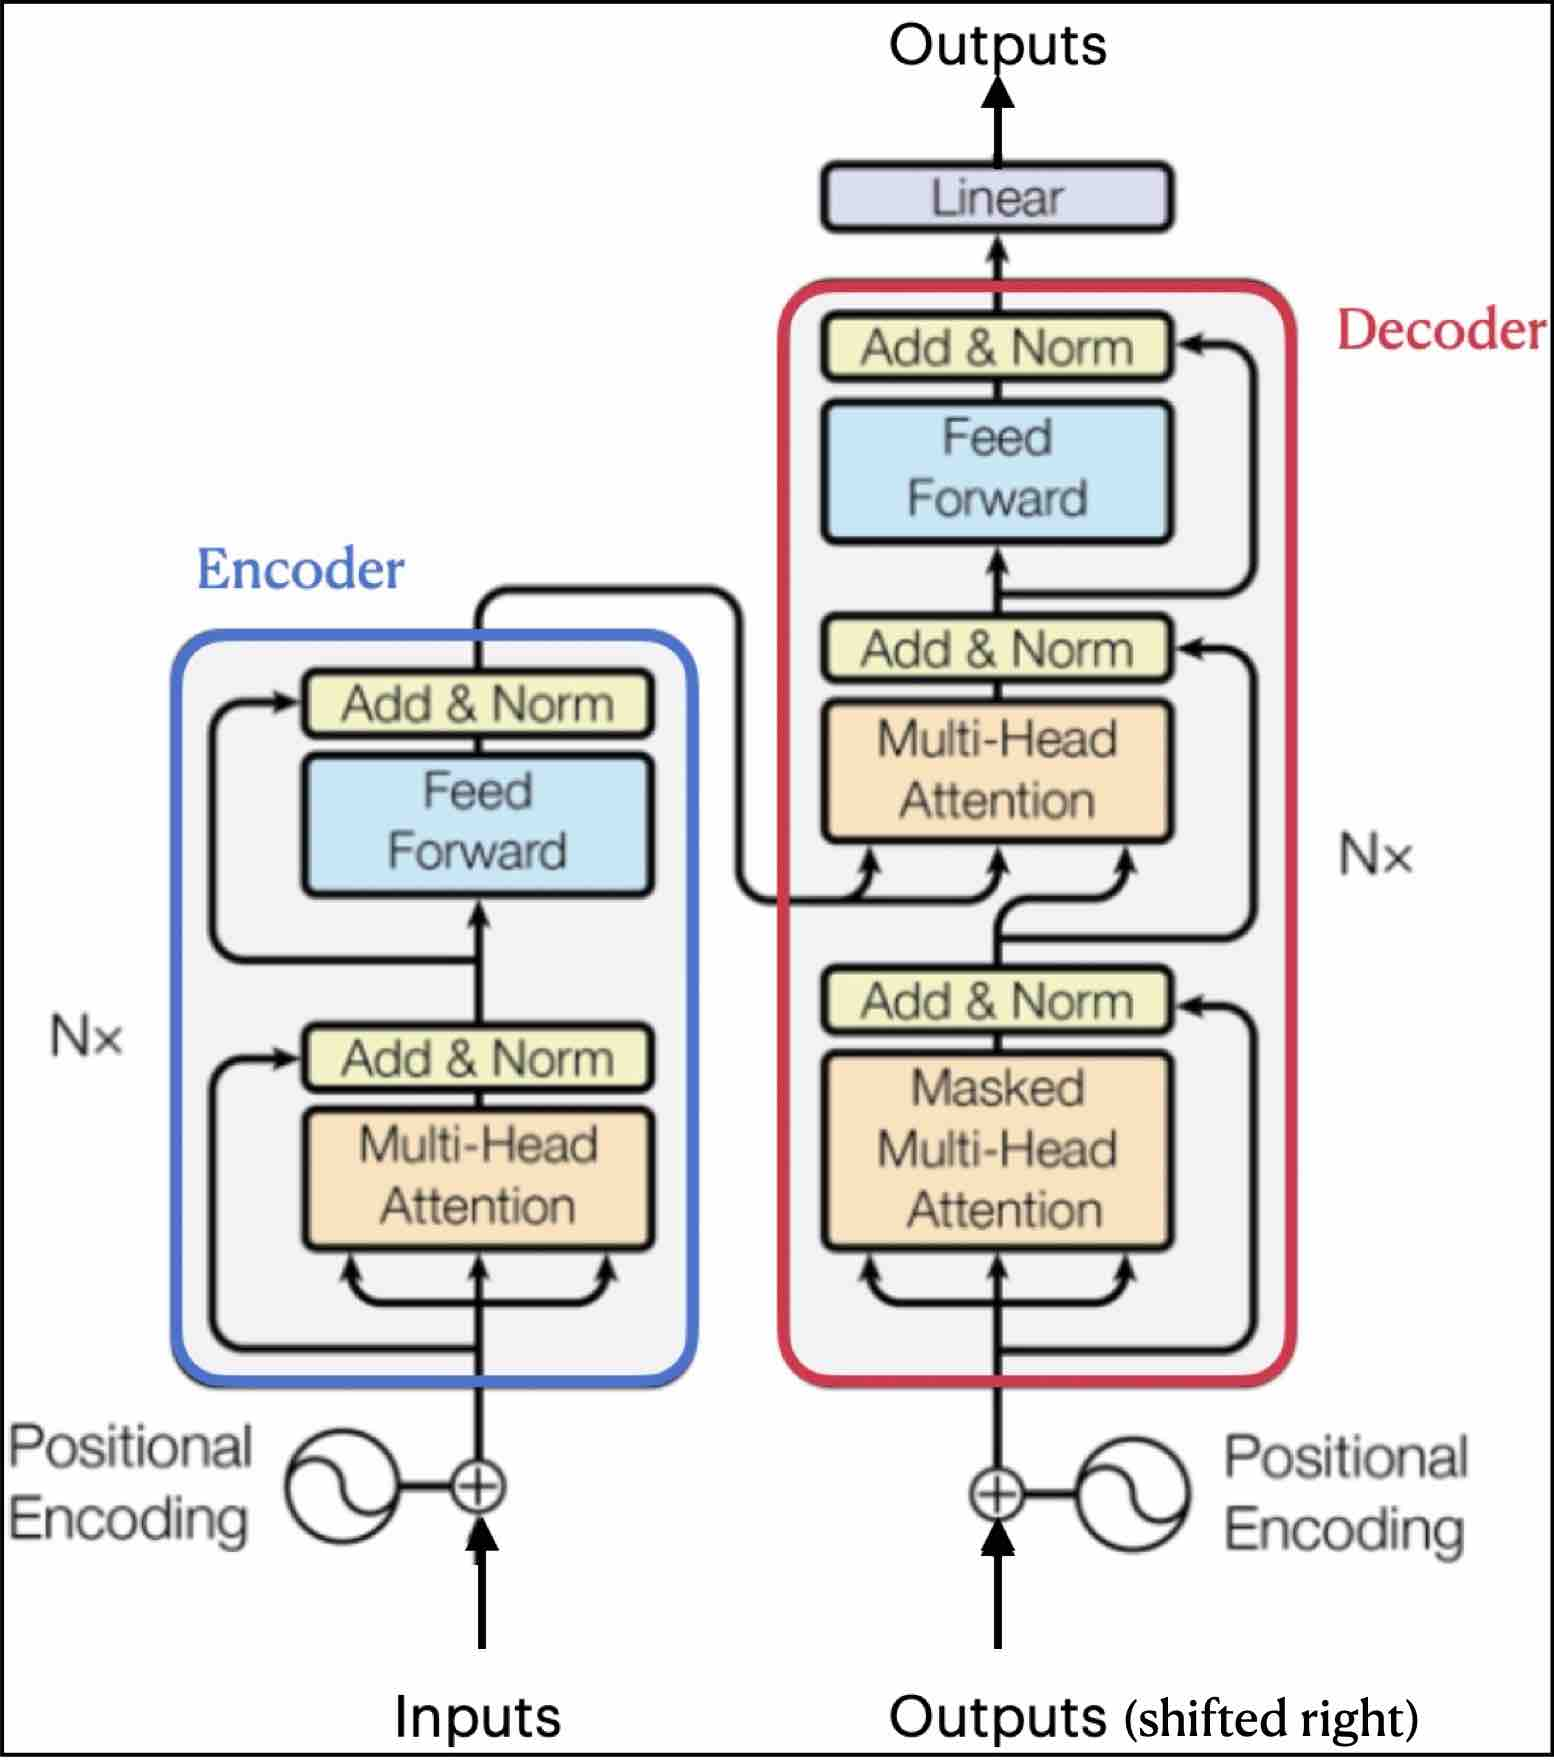
\includegraphics[scale = 0.22]{figures/transformer_metho.jpg}
\end{figure}

\section{Evaluation Plan}

To assess the performance of the model, the model will be tested on untrained activities such as jumping and dropping the ball at different positions around the installed system. The preferred accuracy should be a 75\% hit rate for anomalous events. 
% and less than 5 false positive per day.

\FloatBarrier